% generated by Plantuml 1.2022.7       
\definecolor{plantucolor0000}{RGB}{241,241,241}
\definecolor{plantucolor0001}{RGB}{24,24,24}
\definecolor{plantucolor0002}{RGB}{180,167,229}
\definecolor{plantucolor0003}{RGB}{0,0,0}
\definecolor{plantucolor0004}{RGB}{132,190,132}
\definecolor{plantucolor0005}{RGB}{3,128,72}
\definecolor{plantucolor0006}{RGB}{173,209,178}
\definecolor{plantucolor0007}{RGB}{200,41,48}
\definecolor{plantucolor0008}{RGB}{254,255,221}
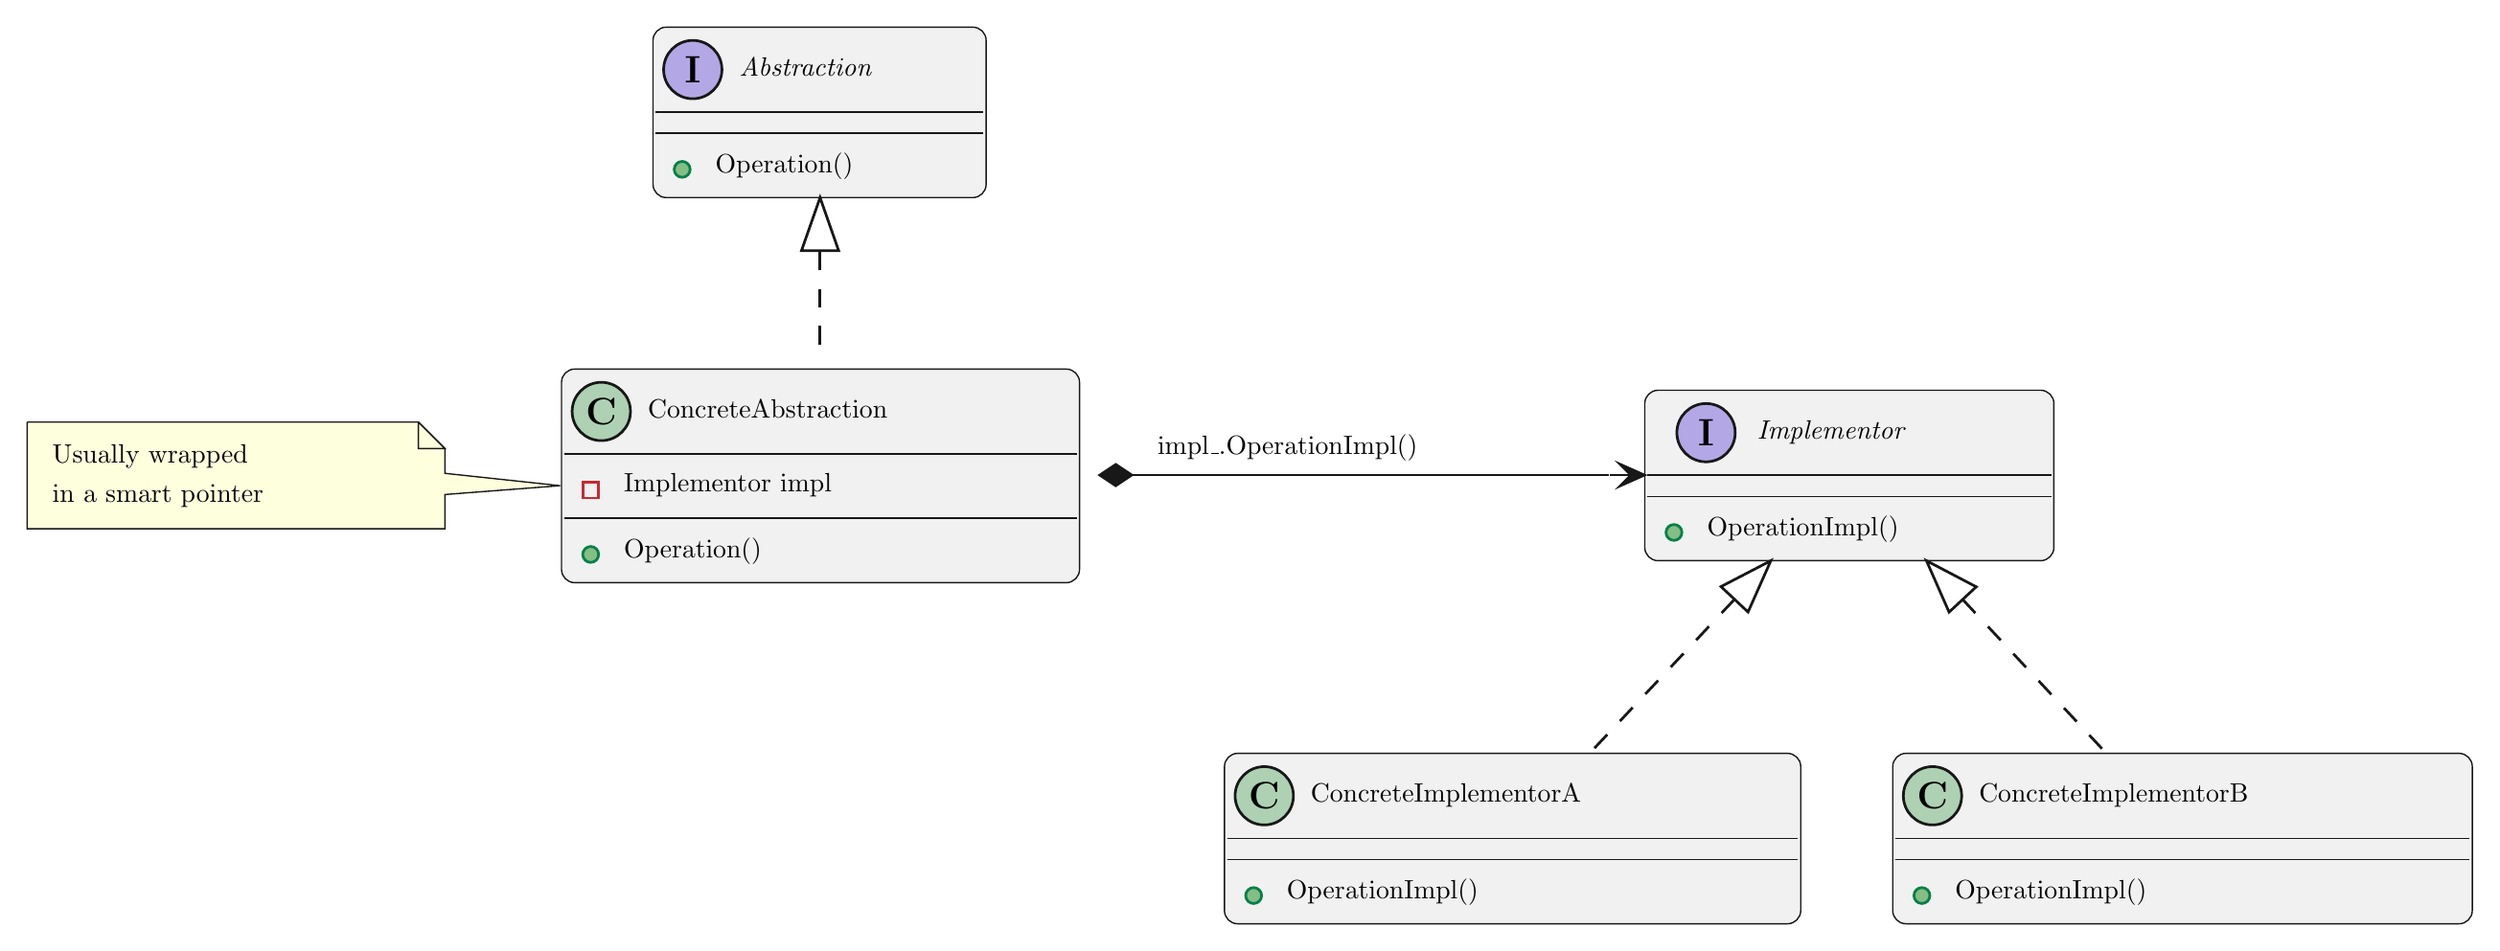
\begin{tikzpicture}[yscale=-1
,pstyle0/.style={color=plantucolor0001,fill=plantucolor0000,line width=0.5pt}
,pstyle1/.style={color=plantucolor0001,fill=plantucolor0002,line width=1.0pt}
,pstyle2/.style={color=plantucolor0001,line width=0.5pt}
,pstyle3/.style={color=plantucolor0005,fill=plantucolor0004,line width=1.0pt}
,pstyle4/.style={color=plantucolor0001,fill=plantucolor0006,line width=1.0pt}
,pstyle6/.style={color=plantucolor0001,fill=plantucolor0008,line width=0.5pt}
,pstyle7/.style={color=plantucolor0001,line width=1.0pt,dash pattern=on 7.0pt off 7.0pt}
,pstyle8/.style={color=plantucolor0001,line width=1.0pt}
,pstyle9/.style={color=plantucolor0001,fill=plantucolor0001,line width=1.0pt}
]
\draw[pstyle0] (242pt,12pt) arc (180:270:5pt) -- (247pt,7pt) -- (362.6195pt,7pt) arc (270:360:5pt) -- (367.6195pt,12pt) -- (367.6195pt,66.2969pt) arc (0:90:5pt) -- (362.6195pt,71.2969pt) -- (247pt,71.2969pt) arc (90:180:5pt) -- (242pt,66.2969pt) -- cycle;
\draw[pstyle1] (257pt,23pt) ellipse (11pt and 11pt);
\node at (257pt,23pt)[]{\textbf{\Large I}};
\node at (271pt,14.8516pt)[below right,color=black]{\textit{Abstraction}};
\draw[pstyle2] (243pt,39pt) -- (366.6195pt,39pt);
\draw[pstyle2] (243pt,47pt) -- (366.6195pt,47pt);
\draw[pstyle3] (253pt,60.6484pt) ellipse (3pt and 3pt);
\node at (262pt,51pt)[below right,color=black]{Operation()};
\draw[pstyle0] (207.5pt,141pt) arc (180:270:5pt) -- (212.5pt,136pt) -- (397.8388pt,136pt) arc (270:360:5pt) -- (402.8388pt,141pt) -- (402.8388pt,211.5938pt) arc (0:90:5pt) -- (397.8388pt,216.5938pt) -- (212.5pt,216.5938pt) arc (90:180:5pt) -- (207.5pt,211.5938pt) -- cycle;
\draw[pstyle4] (222.5pt,152pt) ellipse (11pt and 11pt);
\node at (222.5pt,152pt)[]{\textbf{\Large C}};
\node at (236.5pt,143.8516pt)[below right,color=black]{ConcreteAbstraction};
\draw[pstyle2] (208.5pt,168pt) -- (401.8388pt,168pt);
\draw[color=plantucolor0007,line width=1.0pt] (215.5pt,178.6484pt) rectangle (221.5pt,184.6484pt);
\node at (227.5pt,172pt)[below right,color=black]{Implementor impl};
\draw[pstyle2] (208.5pt,192.2969pt) -- (401.8388pt,192.2969pt);
\draw[pstyle3] (218.5pt,205.9453pt) ellipse (3pt and 3pt);
\node at (227.5pt,196.2969pt)[below right,color=black]{Operation()};
\draw[pstyle0] (616pt,149pt) arc (180:270:5pt) -- (621pt,144pt) -- (765.2726pt,144pt) arc (270:360:5pt) -- (770.2726pt,149pt) -- (770.2726pt,203.2969pt) arc (0:90:5pt) -- (765.2726pt,208.2969pt) -- (621pt,208.2969pt) arc (90:180:5pt) -- (616pt,203.2969pt) -- cycle;
\draw[pstyle1] (639.1027pt,160pt) ellipse (11pt and 11pt);
\node at (639.1027pt,160pt)[]{\textbf{\Large I}};
\node at (654.9032pt,151.8516pt)[below right,color=black]{\textit{Implementor}};
\draw[pstyle2] (617pt,176pt) -- (769.2726pt,176pt);
\draw[pstyle2] (617pt,184pt) -- (769.2726pt,184pt);
\draw[pstyle3] (627pt,197.6484pt) ellipse (3pt and 3pt);
\node at (636pt,188pt)[below right,color=black]{OperationImpl()};
\draw[pstyle0] (457.5pt,286pt) arc (180:270:5pt) -- (462.5pt,281pt) -- (669.8102pt,281pt) arc (270:360:5pt) -- (674.8102pt,286pt) -- (674.8102pt,340.2969pt) arc (0:90:5pt) -- (669.8102pt,345.2969pt) -- (462.5pt,345.2969pt) arc (90:180:5pt) -- (457.5pt,340.2969pt) -- cycle;
\draw[pstyle4] (472.5pt,297pt) ellipse (11pt and 11pt);
\node at (472.5pt,297pt)[]{\textbf{\Large C}};
\node at (486.5pt,288.8516pt)[below right,color=black]{ConcreteImplementorA};
\draw[pstyle2] (458.5pt,313pt) -- (673.8102pt,313pt);
\draw[pstyle2] (458.5pt,321pt) -- (673.8102pt,321pt);
\draw[pstyle3] (468.5pt,334.6484pt) ellipse (3pt and 3pt);
\node at (477.5pt,325pt)[below right,color=black]{OperationImpl()};
\draw[pstyle0] (709.5pt,286pt) arc (180:270:5pt) -- (714.5pt,281pt) -- (923.0557pt,281pt) arc (270:360:5pt) -- (928.0557pt,286pt) -- (928.0557pt,340.2969pt) arc (0:90:5pt) -- (923.0557pt,345.2969pt) -- (714.5pt,345.2969pt) arc (90:180:5pt) -- (709.5pt,340.2969pt) -- cycle;
\draw[pstyle4] (724.5pt,297pt) ellipse (11pt and 11pt);
\node at (724.5pt,297pt)[]{\textbf{\Large C}};
\node at (738.5pt,288.8516pt)[below right,color=black]{ConcreteImplementorB};
\draw[pstyle2] (710.5pt,313pt) -- (927.0557pt,313pt);
\draw[pstyle2] (710.5pt,321pt) -- (927.0557pt,321pt);
\draw[pstyle3] (720.5pt,334.6484pt) ellipse (3pt and 3pt);
\node at (729.5pt,325pt)[below right,color=black]{OperationImpl()};
\draw[pstyle6] (6pt,156pt) -- (6pt,196.2656pt) -- (163.5391pt,196.2656pt) -- (163.5391pt,183.34pt) -- (207pt,180pt) -- (163.5391pt,175.34pt) -- (163.5391pt,166pt) -- (153.5391pt,156pt) -- (6pt,156pt);
\draw[pstyle6] (153.5391pt,156pt) -- (153.5391pt,166pt) -- (163.5391pt,166pt) -- (153.5391pt,156pt);
\node at (12pt,161pt)[below right,color=black]{Usually wrapped};
\node at (12pt,176.1328pt)[below right,color=black]{in a smart pointer};
\draw[pstyle7] (305pt,91.74pt) ..controls (305pt,104.99pt) and (305pt,119.09pt) .. (305pt,131.84pt);
\draw[pstyle8] (298pt,91.31pt) -- (305pt,71.31pt) -- (312pt,91.31pt) -- (298pt,91.31pt) -- cycle;
\draw[pstyle7] (649.79pt,222.93pt) ..controls (631.83pt,242.02pt) and (611.46pt,263.68pt) .. (595.3pt,280.86pt);
\draw[pstyle8] (644.74pt,218.08pt) -- (663.54pt,208.31pt) -- (654.94pt,227.67pt) -- (644.74pt,218.08pt) -- cycle;
\draw[pstyle7] (735.87pt,222.93pt) ..controls (753.69pt,242.02pt) and (773.9pt,263.68pt) .. (789.93pt,280.86pt);
\draw[pstyle8] (730.75pt,227.71pt) -- (722.22pt,208.31pt) -- (740.99pt,218.16pt) -- (730.75pt,227.71pt) -- cycle;
\draw[pstyle8] (422.51pt,176pt) ..controls (422.51pt,176pt) and (549.3pt,176pt) .. (602.6pt,176pt);
\draw[pstyle9] (615.82pt,176pt) -- (606.82pt,172pt) -- (610.82pt,176pt) -- (606.82pt,180pt) -- (615.82pt,176pt) -- cycle;
\draw[pstyle8] (610.82pt,176pt) -- (602.82pt,176pt);
\draw[pstyle9] (410.51pt,176pt) -- (416.51pt,180pt) -- (422.51pt,176pt) -- (416.51pt,172pt) -- (410.51pt,176pt) -- cycle;
\node at (428.75pt,157pt)[below right,color=black]{impl\_.OperationImpl()};
\end{tikzpicture}
